% chapter2 基础

\chapter{运动想象脑电图分类和深度神经网络基础}

\section{脑电生理基础}

\subsection{人脑结构与运动想象}

大脑作为神经活动的中枢处理器,其活动产生的多元生物电信号揭示了人体的认知行为、感官体验、情绪调控等多种思维活动和行动指令。通过现代神经科学技术,如脑电图(EEG)、功能性磁共振成像(fMRI)、近红外光谱成像(NIRS)等手段,人类能够探测并解读这些生物信号,从而了解大脑内部的运作机制。

大脑皮层是大脑最外部的灰质结构,承载了复杂的高级认知功能。大脑皮层中与运动相关的结构主要包括初级运动皮层(Primary Motor Cortex, M1)、辅助运动区(Supplementary Motor Area, SMA)、运动前区(Premotor Cortex,PMC)、顶叶皮层(Parietal Lobe)、前额叶皮层(Prefrontal Lobe,PFC),此外,位于基底神经节的纹状体(Striatum)也参与其中。运动想象(Motor Imagery, MI)是一种心理活动,指的是在没有实际执行肢体运动的情况下,个体在脑海中模拟或重现某项运动的过程,研究发现,当个体执行运动想象任务时,这些脑区仍然会有激活,其中,主要激活的是辅助运动区,辅助运动区在运动执行任务以及运动想象任务中与运动前区、感觉运动皮层区、默认网络结构都存在双向连接\cite{solodkin2004fine},并且存在指向纹状体的单向连接\cite{watanabe2015effects}。相对于运动执行任务,运动想象任务中主运动皮层也存在激活,但激活程度不及运动执行任务\cite{solodkin2004fine}\cite{kasess2008suppressive}。大脑皮层中各运动区的位置如图~\ref{fig:brain}~\cite{penfield1950cerebral}所示。
\begin{figure}
    \centering
    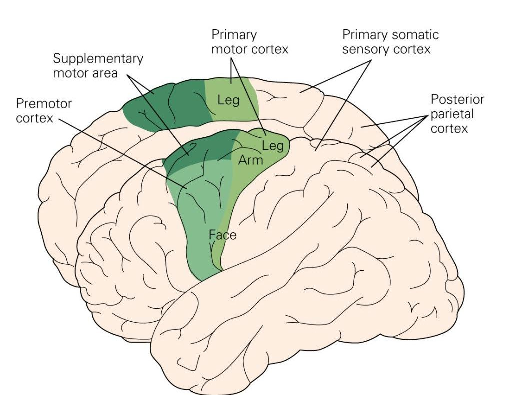
\includegraphics[width=0.4\textwidth]{brain.pdf}
    \caption{大脑皮层运动相关区域}
    \label{fig:brain}
\end{figure}

\subsection{脑电图信号及其特性}

脑电图信号(Electroencephalogram,EEG)由皮质内大量神经元突触后电位同步总和形成,是很多神经元共同活动的结果\cite{ZWQX201803022}。EEG信号可以分为深部EEG,皮层EEG和头皮EEG\cite{1022779250.nh}。相比深部EEG和皮层EEG,从头皮采集的EEG信号需穿透颅骨和头皮组织,因此具有相对较低的信号质量,但头皮EEG无需进行任何开创性手术,极大地降低了医疗风险,保证了高度的安全性,并且实施便捷,获取数据更为简易。因此,头皮EEG成为了神经系统疾病诊断、脑功能研究等领域广泛应用的首选工具。后文中所提到的EEG信号,如无特殊说明,都是指头皮EEG。

EEG信号的采集设备为脑电采集系统,其样式如图~\ref{fig:equip}~所示,通过在受试者头皮上放置单个或多个脑电极(或称通道),以连续、实时的方式记录一段时间内的大脑皮层产生的电信号。图~\ref{fig:montage}~展示了脑电极在头皮上的一种排列方式。EEG信号的采集方式决定了其数据的形状,通常为脑电极(通道)与时间构成的二维数据,其可视化如图所示。对于单通道采集的数据,EEG信号可视化以电位为纵轴,时间为横轴,表示该通道上电位随时间的变化,图~\ref{fig:eeg}~为包含16个通道的EEG信号可视化,可视化中相邻的通道在空间上未必具有相邻关系。
\begin{figure}[h]
    \centering
    \begin{subfigure}{0.4\textwidth}
      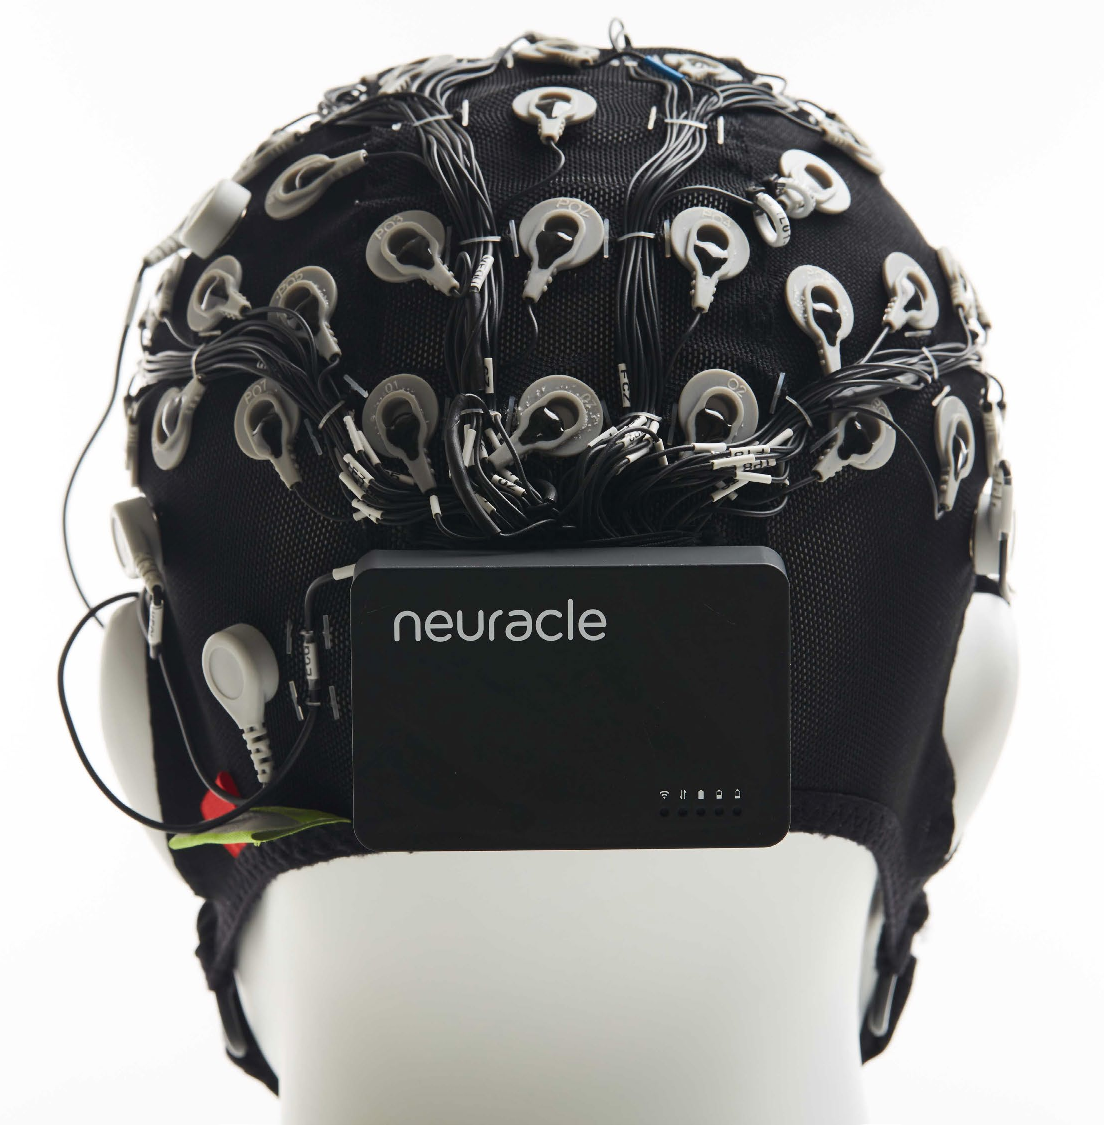
\includegraphics[width=\linewidth]{equip.pdf}
      \caption{脑电采集设备}
      \label{fig:equip}
    \end{subfigure}\qquad
    \begin{subfigure}{0.4\textwidth}
      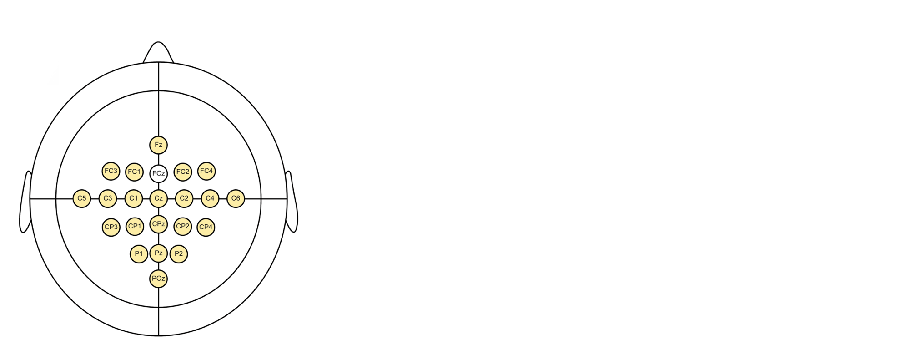
\includegraphics[width=\linewidth]{montage.pdf}
      \caption{一种脑电极排列方式}
      \label{fig:montage}
    \end{subfigure}
    \caption{脑电信号采集}
    \label{fig:eeg-cap}
  \end{figure}
\begin{figure}
    \centering
    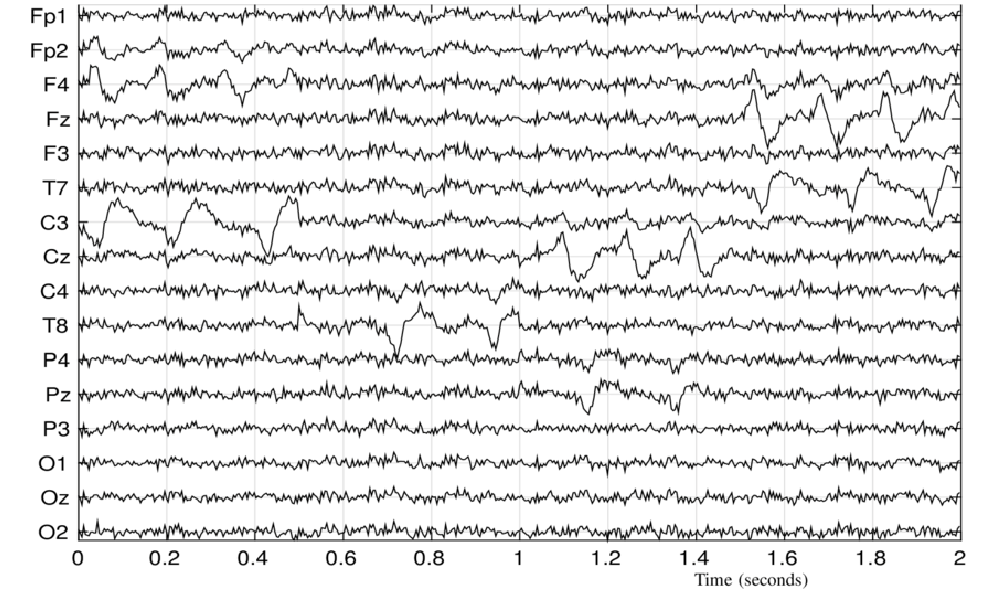
\includegraphics[width=0.8\textwidth]{eeg.pdf}
    \caption{EEG信号可视化}
    \label{fig:eeg}
\end{figure}

正常脑电信号是多个具有生物学意义的神经振荡节律的组合\cite{1022779250.nh}。神经科学研究发现,根据脑电信号的频率范围可以划分出五种主要节律:

(1) Delta:频率范围为0.5-4Hz。研究发现,Delta波的起源主要有两个,分别是皮层和丘脑,后者主要与睡眠相关\cite{kropotov2010quantitative}。Delta节律主要出现在深度睡眠阶段,尤其是在儿童和婴儿的脑电图中尤为明显。成年人在某些病理状态下也可观察到增强的Delta节律,如严重的器质性脑疾病。

(2) Theta:频率范围为4-8Hz。Theta节律不仅出现在轻度睡眠和快速眼动睡眠阶段,还可见于青少年和儿童清醒时的脑电图中,以及成年人在专注、疲劳或焦虑状态下的头顶前部中线位置\cite{ishihara1966activation}\cite{ishihara1967interaction}。

(3) Alpha:频率范围为8-13Hz。Alpha节律依据起源位置的不同可分为两大类:一类是源自初级躯体感觉皮层(Primary Somatosensory Cortex, S1)的Mu节律(或称运动Alpha节律)\cite{hari1997human},手部运动、运动想象等活动可以阻断Mu节律,而在肌肉放松状态下则会增强Mu节律;另一类则是来源于视觉皮层或枕叶的Alpha节律,通常在个体放松、闭眼精细状态出现,而在睁眼或注意力集中时受到抑制,表现为振幅减小。此外,有研究指出,脑力劳动的增加也将导致Alpha节律活动的减弱\cite{1022779250.nh}。

(4) Beta:频率范围为13-30Hz。Beta节律根据分布区域的不同可分为两大类:一类是在感觉运动皮层区域表现最强的运动Beta节律(Rolandic Beta),其活动强度受运动任务影响,在运动想象、运动准备和运动执行过程中,Rolandic Beta节律的幅值功率都会有相应变化;另一类是在额叶区域表现最强的额叶Beta节律(Frontal Beta),此类节律主要出现在清醒、警觉、专注以及执行认知任务时的大脑活动中,其强度的增加通常与认知活动和心理负荷的上升相关联。

(5) Gamma:频率范围通常定义为超过30Hz,有时也指25Hz至100Hz甚至更高的频率范围。Gamma节律广泛参与到认知处理、意识维持、注意力集中、感知整合和记忆编码等复杂脑功能过程中,被认为与高级认知功能和信息整合紧密相关。Gamma节律可在多个脑区观察到,包括但不限于前额叶、顶叶和颞叶区域。

需要说明的是,各类脑电波的频率范围并不是绝对分割的,而是存在着一定的重叠与交织。在实际的大脑生理活动中,某一时刻或时间段内的脑电信号往往包含了多种不同的节律形态,不仅限于Delta、Theta、Alpha、Beta、Gamma五类,例如,Rolandic Beta节律和Frontal Beta节律可以同时出现。实际上,脑电极采集到的脑电信号通常是不同频率节律相互交织、叠加而成的复杂组合。

除却具有脑生理活动信息的EEG节律,脑电极会同时采集到各类噪声信息,称之为EEG伪迹。常见的EEG伪迹有以下几种:

(1) 眼动伪迹:当眼睛移动(如眨眼、扫视等)时,眼周的肌肉和眼睑的电位变化会在电极上产生强烈的电位波动。这种伪迹在额部电极附近特别明显,特征是突然出现的尖峰或方波形状的电位变化。眼动信号可以通过眼电图(Electrooculogram,EOG)记录。EOG的幅度一般是EEG信号的几倍,频率通常分布在3-16Hz,幅值通常分布在0.5-4mV。

(2) 肌电伪迹:肌电伪迹主要来自于头颈部及面部肌肉的伸展和收缩,如吞咽、呼吸、讲话等。肌电伪迹通常表现为高频、大振幅的波动,与实际脑电活动相比更加剧烈和不稳定。肌电信号可以通过肌电图(Electromyogram,EMG)记录。EMG的频率在0-200Hz广泛分布。

(3) 心电伪迹:脑电极分布在脑部血管附近,心脏搏动会在头皮电极上产生明显的电位波动,尤其是在靠近耳朵后部的乳突区域。心电伪迹通常表现为周期性出现的正弦波形,与心脏搏动频率(大约每分钟60-100次)相符。心电信号可以通过心电图(Electrocardiogram,ECG)记录。ECG的波形类似EEG波形,频率在0.05-100Hz广泛分布。

(4) 工频伪迹:工频干扰来源于电源线和其他电气设备释放的50Hz(欧洲和亚洲大部分地区)或60Hz(北美和其他部分地区)的交流电噪声。这种干扰在EEG信号中表现为稳定的、与电源频率相同的周期性波动。

为了减少EEG信号中的伪迹干扰,通常会在数据预处理阶段运用一系列针对性算法和技术。例如,利用独立成分分析识别并排除源于眼动和肌电活动的伪迹成分,通过低通滤波抑制心电伪迹在特定频率范围内的影响等。然而,需要说明的是,即便是基于信号处理技术和神经科学先验知识,伪迹的去除过程仍有可能导致某种程度的真实脑电信息丢失。尤其是在处理复杂、微妙的脑电活动时,很难做到既能彻底清除伪迹又不损害有价值信号的完整性。

综上所述,EEG信号是一种蕴含丰富信息却又存在诸多问题的复杂生物电信号,它不仅涵盖着从Delta至Gamma等多种频率范围的脑电节律,且这些节律在实际记录中存在交错重叠的现象。此外,EEG信号容易受到多种噪声源的显著影响,包括眼动伪迹、肌电伪迹、心电伪迹等生理伪迹以及工频干扰等非生理伪迹。鉴于EEG信号的独特生理特征和采集特点,它展现出一些鲜明的特性:

(1) 低信号强度。EEG信号采集的是神经元活动产生的微弱电压波动,其强度一般在\(\mu\)V级别(5-100\(\mu\)V)\cite{SJCJ201505001}。这使EEG信号易受噪声影响,提高了信号处理和解析的难度。

(2) 宽带特性,低信噪比。EEG信号所蕴含的有价值信息具有显著的时间动态性,即这些信息会随时间持续演变并在整个时间域内传播,这使得EEG信号在频谱分析中呈现出宽广的频率范围,其中包含的主要成分通常分布在大约0.5至45Hz的频率范围内\cite{1022779250.nh},涵盖了Delta、Theta、Alpha、Beta及部分Gamma节律。然而,由于伪迹噪声普遍存在且分布广泛,EEG信号中蕴含的有用信息时常与伪迹及其他信息在不同频带上相互交叉混叠。与此同时,由于人体脑电信号本身强度微弱,加之复杂的生理和心理状态变化,以及检测技术在实际应用中的不稳定性,进一步导致了在实际采集的EEG信号数据中,不同脑电成分之间易于互相干扰和混淆。这些现象显著降低了EEG信号的信噪比,即有用信号与噪声的比例较低。这为EEG信号的分析带来了困难,难以完整地将有用信号从背景噪声中剥离,并且需要依赖经验和神经科学先验知识,耗费相当的开销。

(3) 非平稳性,被试特异性。不同于平稳随机信号,EEG信号的统计特性随时间发生变化,其频率、幅度等特征在不同任务条件下呈现出显著的动态变化,表明EEG信号具有明显的非平稳性。与此同时,不同个体(被试)所产生的EEG信号在频率成分、幅度强度、响应时间等方面通常表现出个体间的差异性;不仅如此,即使是同一被试在不同时间段内执行同样的任务,其所产生的EEG信号也可能存在变化。因此,EEG信号具有显著的被试特异性(Subject-Specificity),意味着每位被试的脑电活动模式在很大程度上是个体独有的。这使得很难使用一种固定的方法对EEG信号进行分析。

(4) 非线性。EEG信号不是单一过程的结果,而是多种脑内过程或同源过程非线性耦合与叠加的产物,呈现出显著的非线性特征。这种非线性特性使得各种信号成分之间的相互作用和影响更为复杂化,极大地提升了EEG信号分析的复杂度和解析难度。

(5) 多通道,时空分布不均。在实际采集过程中,EEG信号通常利用多个脑电极(通道)进行同步记录,形成了多通道数据属性。同时,EEG信号的时空分布不均匀,大脑在执行特定功能时,会在特定时间和脑区产生显著的电压波动,例如,进行眼球运动时,在额部电极附近会产生即时且明显的眼电活动。脑电极的分布通常使用国际10-20标准导联确定,其中,“10”和“20”指相邻电极之间的实际距离设定为头骨前后或左右总距离的10\%或20\%,标准10-20导联系统包含了21个电极,这些电极捕获的信号在不同大脑活动中蕴含的信息量不尽相同。此外,EEG信号在时间域的数据量往往要高于空间域的数据量,且时间域蕴含的有效信息更为丰富。这种时空分布的不均衡性提升了筛选和提取有效信息的困难性。

EEG信号具有时间域、空间域、频率域三个维度的特征。在时间域层面,EEG信号揭示了神经活动随时间推移的动态变化过程;在空间域层面,EEG信号揭示了神经活动在不同头皮电极位置上的强度分布差异,反映了大脑不同区域的功能活动;而在频率域层面,EEG信号反映了信号中蕴含的不同脑电节律。脑电采集设备所采集到的原始EEG信号直观地反映了时间域和空间域的特征,如图~\ref{fig:eeg}~所示。频率域的特征则需要通过快速傅里叶变换等频谱分析技术对原始数据进行转换。相较于直接处理原始的EEG信号,提取频率域特征通常需要更多的计算资源和处理时间,耗费更高的开销。

\subsection{脑电图信号与运动想象}

事件相关去同步化(Event-Related Desynchronization,ERD)和事件相关同步化(Event-Related Synchronization,ERS)是在研究EEG信号过程中发现的两种脑活动现象,它们反映了大脑在特定任务或事件触发后,特定频段脑电活动的动态变化。

(1) 事件相关去同步:ERD是指在执行一项特定的任务,如运动想象或实际运动时,原本在一定频段上占主导地位的同步脑电活动(即电位振荡趋于一致)出现了减少或消失,表现为脑电功率的下降。这一现象通常与大脑皮层的兴奋性增加和特定区域活动增强有关。在运动想象或实际运动时,初级运动皮层和辅助运动区的Alpha节律(Mu节律)、Beta节律通常会出现ERD现象。

(2) 事件相关同步:ERS与ERD相反,是指在特定任务或事件发生后,某一频段的脑电活动同步性增强,表现为脑电功率的升高。ERS可能表示大脑某些区域的活动暂时减少或进入了一种休眠状态,为其他区域的活动让渡资源,或者代表了大脑在执行某些认知或精神任务时的资源重新配置。在运动想象或实际运动时,ERS现象同样出现在Alpha节律(Mu节律)和Beta节律中。

在进行单侧肢体的运动想象任务时,大脑呈现出不对称的激活模式:对侧大脑半球(即与执行想象运动的肢体相对应的脑区)通常会出现更为显著的ERD现象,意味着该区域的特定频段脑电活动强度减弱\cite{pfurtscheller1977event}。与此同时,执行运动想象任务的同侧大脑半球则会出现一定程度的ERS现象。实际上,在运动想象任务结束后的放松阶段,ERS现象更为明显,此时大脑可能在先前活跃区域呈现出电活动同步性的增强,这一现象反映了大脑从运动想象状态向静息状态转变时的活动调整和资源分配。进行左右手运动想象时,脑功率谱密度变化如图~\ref{fig:erders}~所示,当想象左手运动时,大脑皮层右侧(C4电极附近)出现ERD现象,相关区域能量减小;当想象右手运动时,大脑皮层左侧(C3电极附近)出现ERD现象,相关区域能量减小。
\begin{figure}
    \centering
    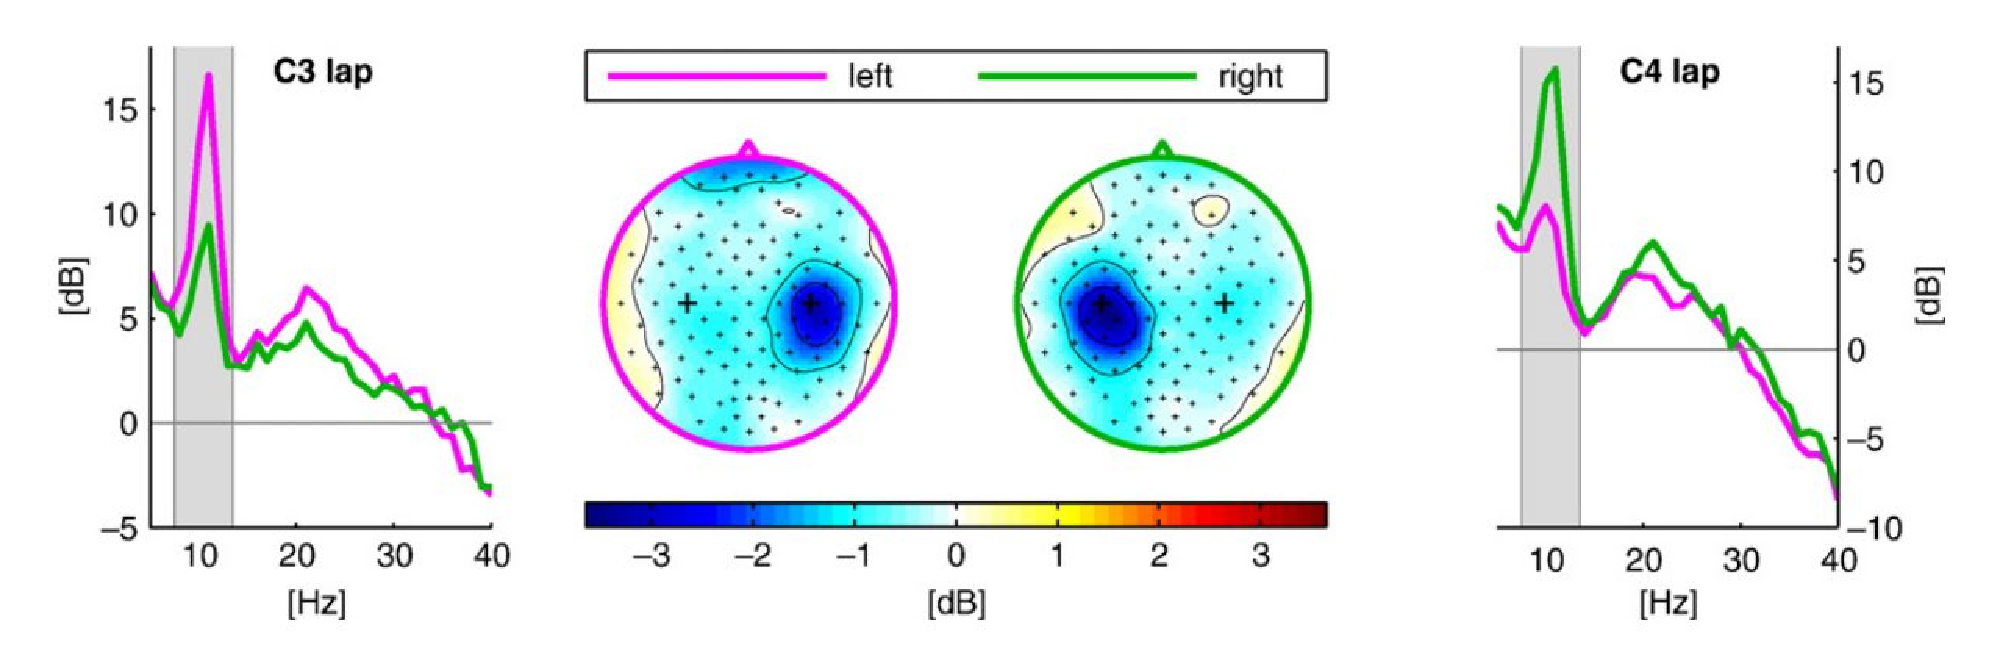
\includegraphics[width=\textwidth]{erders.pdf}
    \caption{左右手运动想象的ERD现象}
    \label{fig:erders}
\end{figure}

综上所述,与运动想象相关的脑电图信号主要是出现在感觉运动皮层的Mu节律和Beta节律,进行运动想象时,主要会出现ERD、ERS这两种脑电活动现象。

\section{深度神经网络基础}

深度神经网络(Deep Neural Network,DNN)是一种模拟人脑神经网络设计的多层非线性模型,在计算机视觉、自然语言处理、语音交互等领域有着广泛的应用。相较于传统的神经网络,深度神经网络通过多个隐藏层逐层对输入数据进行特征提取和抽象,模型复杂度和表达能力显著提高,能够拟合更复杂的非线性关系,取得更为优异的性能和效果。

\subsection{卷积神经网络}

卷积神经网络(Convolutional Neural Network, CNN)是深度学习领域经典且重要的模型,其设计灵感来自于生物学中对动物视觉系统的理解,设计目的是模拟人类的视觉处理过程。CNN在计算机视觉领域取得了巨大成功,广泛应用于图像识别、图像分类、物体检测、语义分割、视频分析等任务中,其优势在于能够自动学习图像特征,无需进行人工特征提取,从而简化了流程,并提高了性能。

CNN的结构主要包括输入层(Input Layer)、卷积层(Convolutional Layer)、池化层(Pooling Layer)、激活函数(ctivation Function)、全连接层(Fully Connected Layer)、输出层(Output Layer),此外还可包括Dropout层、归一化层(Normalization Layer)等。一个简单的用于分类任务的CNN网络结构如图~\ref{fig:cnn}~所示。论文将对其中的重要结构进行说明。
\begin{figure}
    \centering
    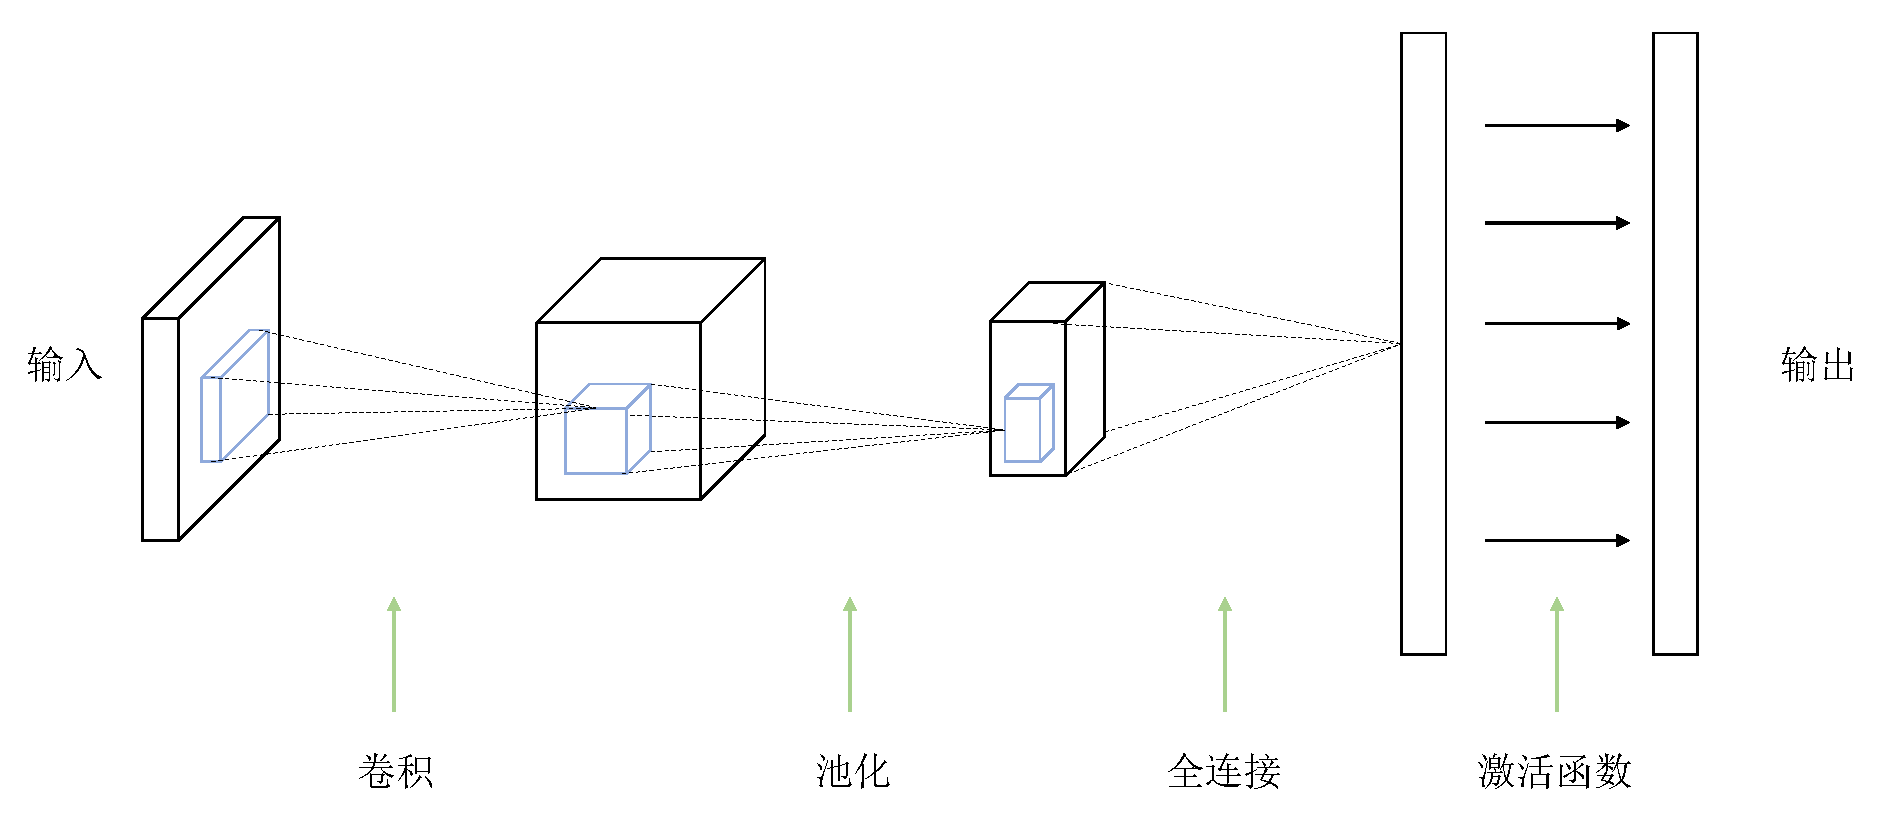
\includegraphics[width=\textwidth]{cnn.pdf}
    \caption{多分类卷积神经网络基本结构}
    \label{fig:cnn}
\end{figure}

(1) 卷积层

(2) 池化层

(3) 激活函数

(4) 归一化层

(5) Dropout层

\subsection{循环神经网络}

\subsection{注意力机制}

\section{基于深度学习的运动想象脑电图分类基础}

\section{本章小结}